\chapter{The Compact Muon Solenoid Experiment}
Located in the shadow of the Jura mountains
at LHC interaction Point 5 is the Compact Muon Solenoid (CMS) Detector. 
The CMS detector is designed with the purpose of detecting and reconstructing
proton-proton and Heavy Ion interactions delivered by the LHC accelerator.
CMS is designed to collect and analyze the full physics reach of the LHC and 
therefore will operate at very high luminosity conditions. Due to the very high
crossing rate (40MHz) and variety of physics processes, very high speed electronics
that have a large set of channels capable of operating in close synchronization are required.

\begin{figure}[t]
  \centering
	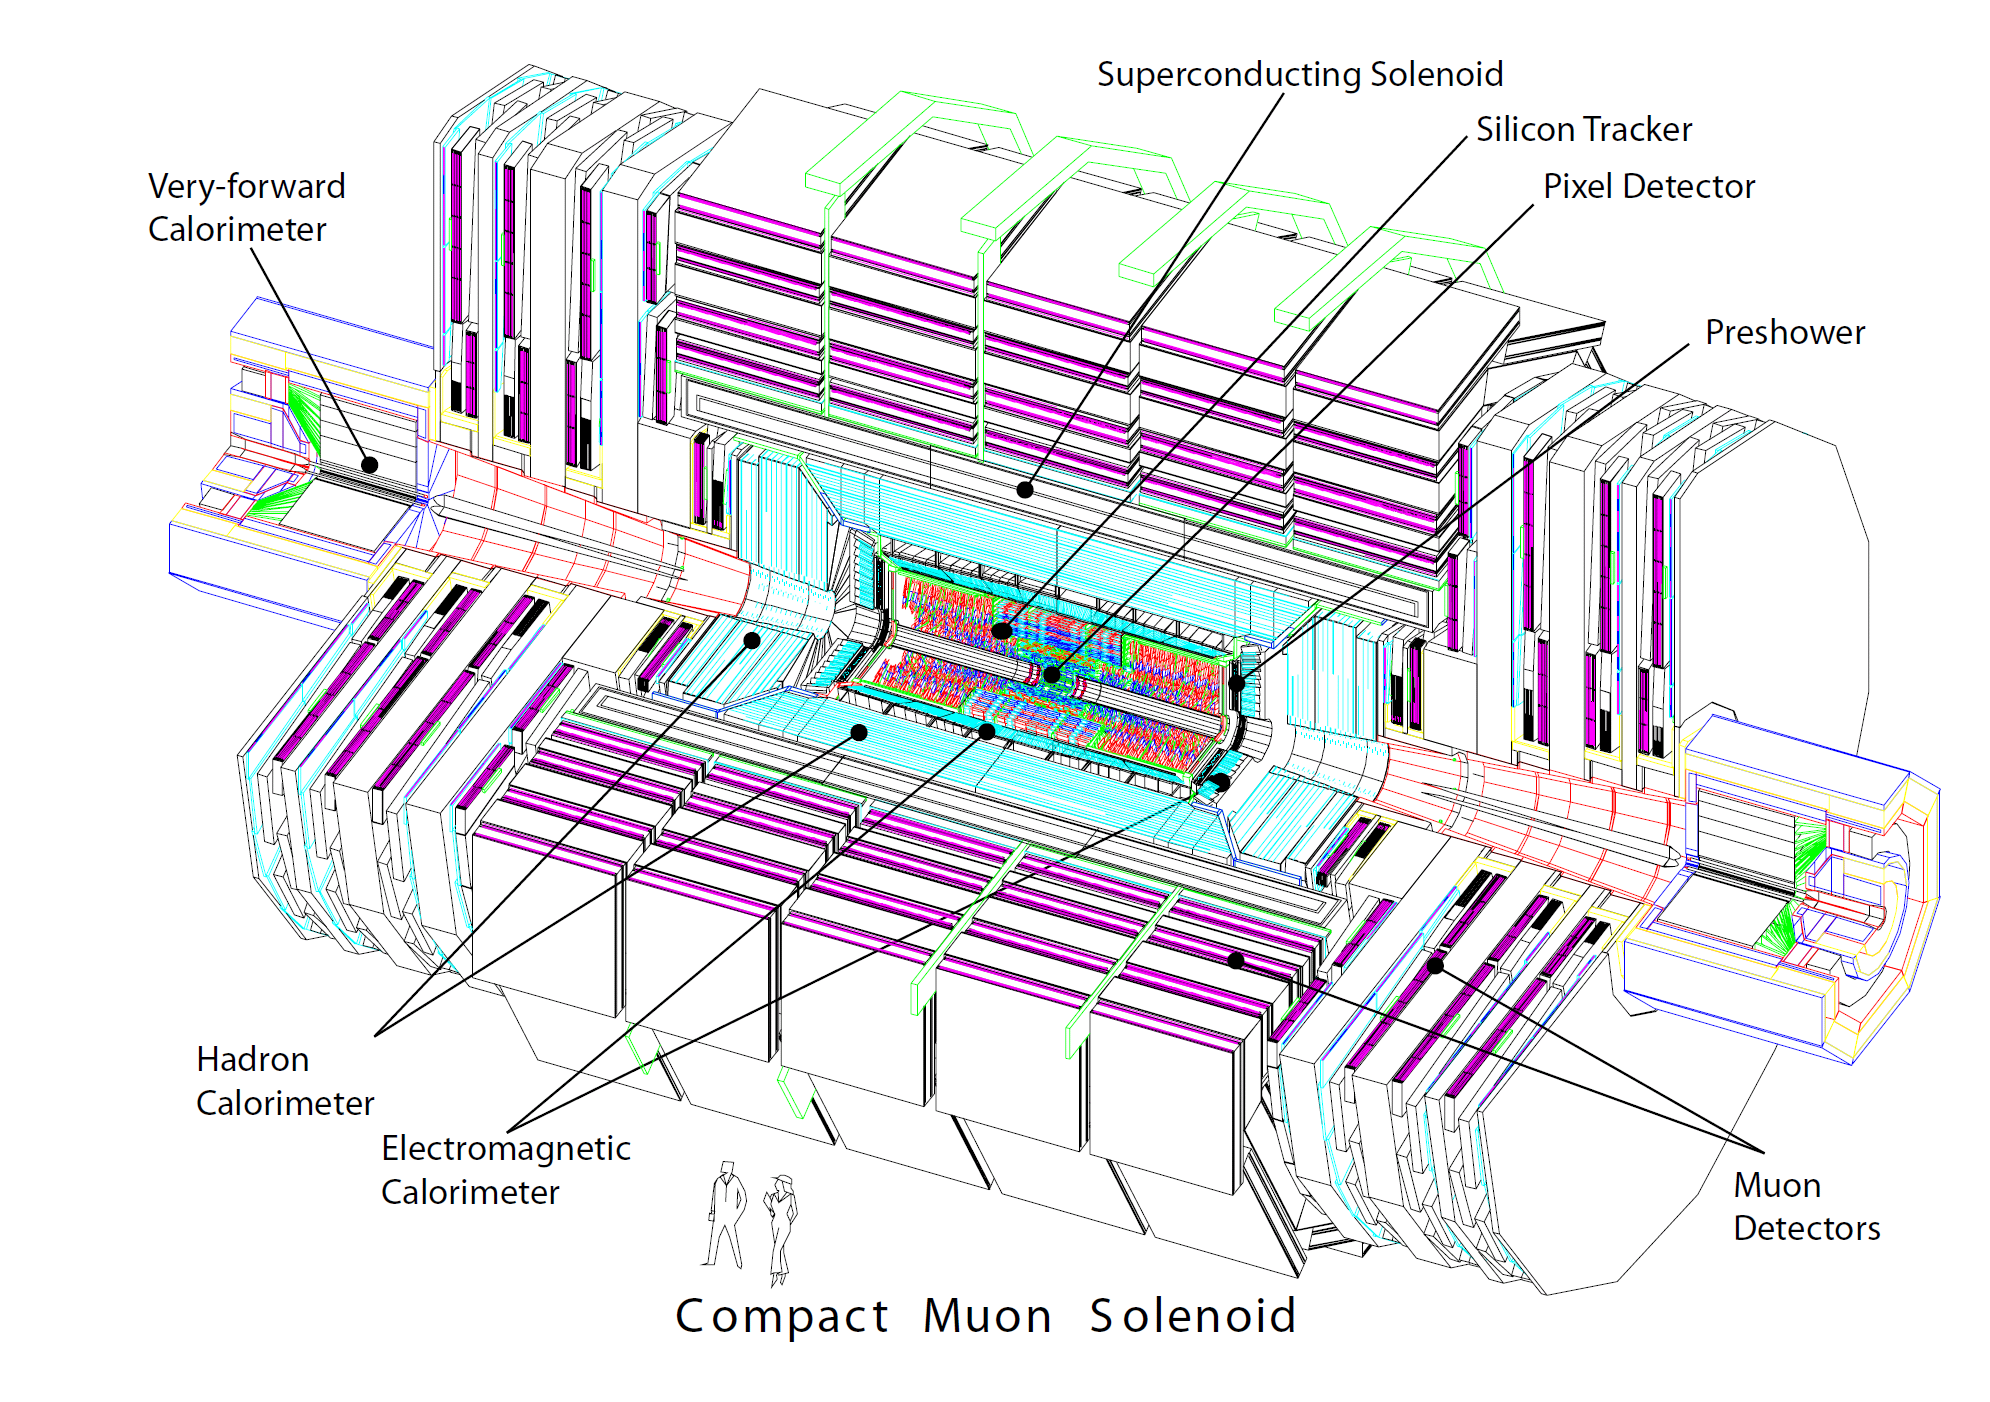
\includegraphics[width=1\textwidth]{images/CMSLayout.png}
  	\caption[CMS Layout]
   	{CMS Layout}
	\label{fig:CMSLayout}
\end{figure}
The CMS detector was designed to meet the following requirements:
\begin{itemize}
\item Good muon identification, momentum resolution asnd charge identification over a wide range of momentum 
\item Good charged particle momentum resolution and reconstruction efficiency within the inner tracker. Efficient
triggering and offline tagging of $\tau$-leptons and b-jets, requiring pixel detectors close to the interaction point
\item Good electromagnetic energy resolution: diphoton and dielectron mass resolution should
be $\approx$1$\%$ at 100 GeV
\item Di-jet mass resolution and missing transverse energy measurement: requires hadron
calorimeters with a wide coverage and fine segmentation
\end{itemize}

To achieve these goals CMS uses a large superconducting solenoid magnet which contains
the silicon tracker (the largest silicon tracker ever built) 
as well as the electromagnetic and hadronic calorimeters;
outside of the solenoid there is an outer hadronic calorimeter
and then the iron magnetic return yoke with multiple layers of muon
detectors installed within it. 
The layout of the detector subsystems and the overall scale of 
CMS can be seen in figure \ref{fig:CMSLayout}.
Their important design features, capabilities and limitations
are detailed in the subsequent sections. 
These detectors and their front-end electronics must be capable of withstanding
large magnetic fields on the order of a few Tesla and
 be able to withstand large doses of radiation (i.e radiation hard). 

Finally, an important and unique aspect of CMS is its moving-ring-based structure,
which is illustrated in figure \ref{fig:CMSMovingRing}.
\begin{figure}[hb]
  \centering
	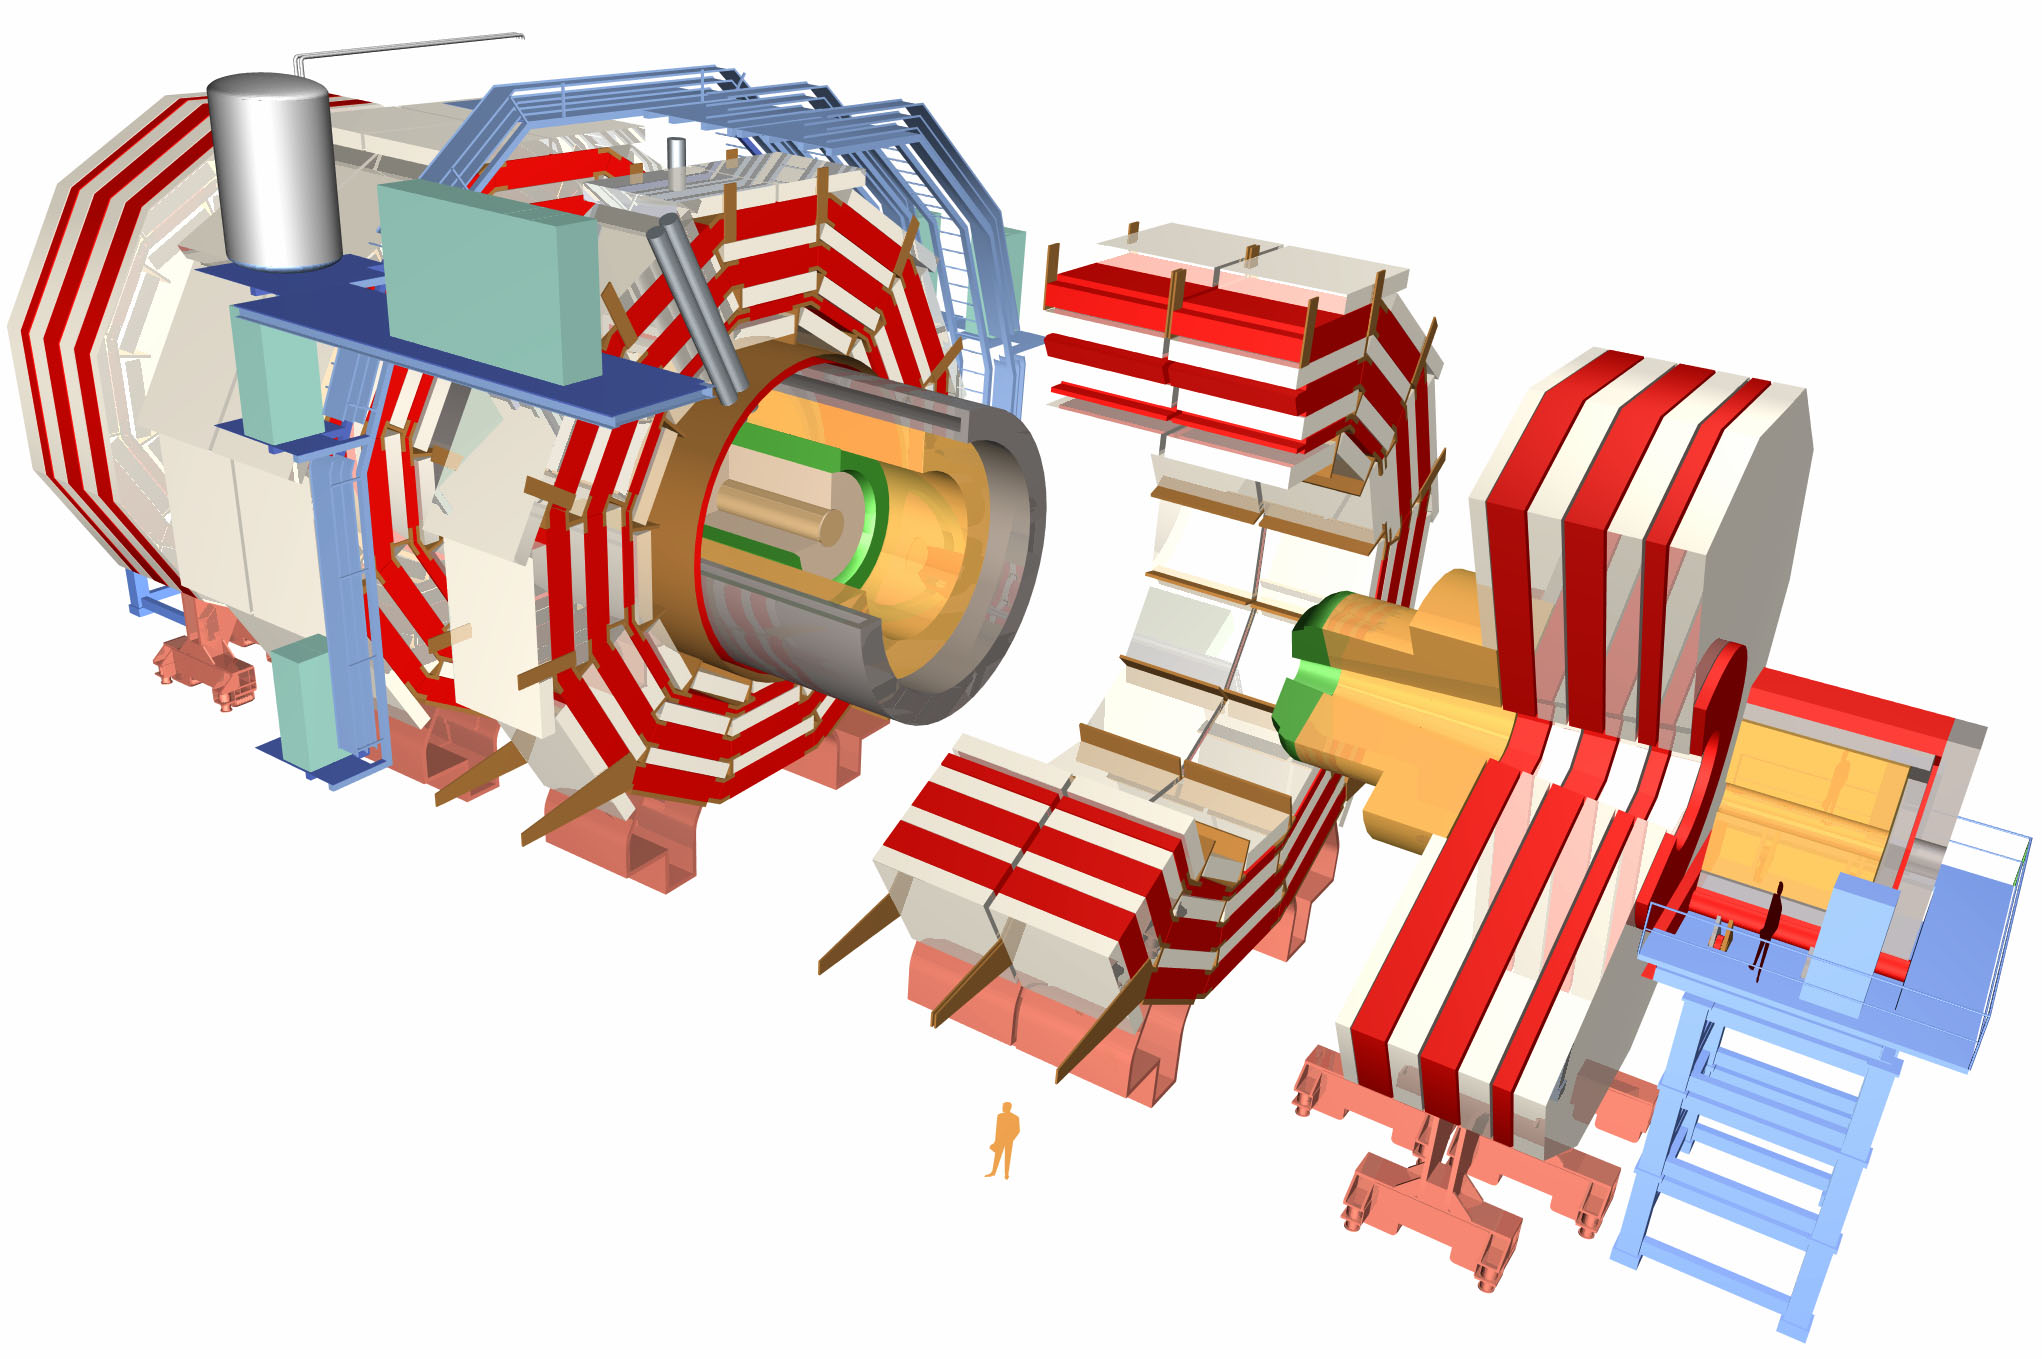
\includegraphics[width=0.7\textwidth]{images/MovingRing.jpg}
  	\caption[Moving Ring Structure]
   	{CMS moving ring structure}
	\label{fig:CMSMovingRing}
\end{figure}
This design choice allows for very good access to the detector elements for 
both maintenance and upgrades which are essential to meeting future running conditions.
